\documentclass[a4paper,12pt]{report}
\usepackage[utf8]{inputenc}
\usepackage[francais]{babel}
\usepackage[T1]{fontenc}
\usepackage{graphicx}
\usepackage{listingsutf8}
\usepackage[colorlinks,urlcolor=blue]{hyperref} %hyperlinks
\usepackage[nottoc,notlot,notlof]{tocbibind} %To bind the table of contents to the bibligoraphy
\usepackage{../../packages/tikz-uml} %UML elements

\begin{document}
%----------------------------------------------------------------------------------------
%   TITLE PAGE
%----------------------------------------------------------------------------------------
\begin{titlepage}
\newcommand{\HRule}{\rule{\linewidth}{0.5mm}} % Defines a new command for the horizontal lines
\center
%----------------------------------------------------------------------------------------
%   LOGOS SECTION
%----------------------------------------------------------------------------------------

\includegraphics[scale=0.5]{images/umLogo.png} % Université de Montpellier Logo
\hspace{\fill}

\includegraphics[scale=0.25]{images/fdsLogo.jpg} % Faculté de Sciences Logo
%----------------------------------------------------------------------------------------
%   HEADING SECTIONS
%----------------------------------------------------------------------------------------
\textsc{\LARGE M1 Informatique AIGLE}\\[1cm]
\textsc{\Large \textbf{HMIN122M}}\\[0.25cm]
\textsc{\large Mini-Projet : entrepôts de données}\\[0.8cm]
%----------------------------------------------------------------------------------------
%   TITLE SECTION
%----------------------------------------------------------------------------------------
\HRule \\[0.4cm]
{ \huge \bfseries Rendu sur la modélisation d'un entrepôts de données}\\[0.4cm]
\HRule \\[0.8cm]
%----------------------------------------------------------------------------------------
%   AUTHORS SECTION
%----------------------------------------------------------------------------------------
\begin{minipage}{\textwidth}
\centering \huge
Bachar \textsc{Rima}\\ % Student
Joseph \textsc{Saba}\\ % Student
Tasnim \textsc{Shaqura Muhammad}\\ % Student
Jérémy \textsc{Bourgin} % Student
\end{minipage} \\[0.8cm]
%----------------------------------------------------------------------------------------
%   DATE SECTION
%----------------------------------------------------------------------------------------
{\large 23 octobre 2018}\\[1cm]
\hspace{\fill}
\vfill % Fill the rest of the page with whitespace
\end{titlepage}

\pagestyle{plain}

{
  \hypersetup{linkcolor=black}
  \tableofcontents
}

\newpage

\chapter*{Introduction}
\label{chap:intro}
\addcontentsline{toc}{chapter}{\nameref{chap:intro}}
Dans le cadre du mini-projet du module \textbf{HMIN122M}, nous avons décidé de modéliser un entrepôts de données pour le réseau de transport publique de Montpellier, \textit{tam-voyages}. Pour ce faire, nous avons proposé des \textit{data marts} formant le \textit{data warehouse} et permettant de réaliser des requêtes analytiques sur un ensemble important de données. Cette modélisation permettra ainsi de mettre en \oe{}uvre un outil d'analyse permettant de bien répondre aux problématiques suivantes :
\begin{enumerate}
  \item Comment \textit{tam-voyages} pourront-ils augmenter leur taux de ventes en se basant sur la circulation du réseau\footnote{en particulier en examinant les lignes de tramway et les bus} ?
  \item Comment \textit{tam-voyages} pourront-ils suivre l'évolution et la maintenance de leurs matériaux de manière à réduire les dépenses qui y sont associées ?
\end{enumerate}

Ces problématiques seront ainsi adressées en analyzant les actions et opérations effectuées par \textit{tam-voyages}, notamment en choisissant celles qui paraissent les plus pertinentes et les plus importantes en termes de données intégrées et flexibilité des critères d'analyse.

\chapter*{Questions}
\label{chap:questions}
\addcontentsline{toc}{chapter}{\nameref{chap:questions}}

\section*{Question 1}
\label{sec:question_1}
\addcontentsline{toc}{section}{\nameref{sec:question_1}}

Les actions/opérations effectuées par \textit{tam-voyages} considérées :
\begin{itemize}
  \item Les voyages.
  \item La maintenance de véhicules.
  \item Les ventes de tickets et les abonnements.
  \item Les amendes.
\end{itemize}

\section*{Question 2}
\label{sec:question_2}
\addcontentsline{toc}{section}{\nameref{sec:question_2}}

\begin{enumerate}
  \item exemples de requêtes analytiques pour l'action \og voyages \fg :
  \begin{itemize}
    \item \texttt{le nombre de voyageurs par bus, utilisant des tickets pour le mois de juillet.}
    \item \texttt{le prix moyen par type de ticket pour chaque voyage pendant les vacances de noël de 2018.}
    \item \texttt{le nombre de voyageurs abonnés par ligne pour chaque voyage pour les deux derniers mois.}
    \item \texttt{l'arrêt le plus fréquenté par toutes les lignes de circulation.}
  \end{itemize}
  \item exemples de requêtes analytiques pour l'action \og maintenance \fg :
  \begin{itemize}
    \item \texttt{le nombre de bus maintenus pour le mois de septembre 2018.}
    \item \texttt{les X premières lignes ayant le nombre maximale de maintenances par mois.}
    \item \texttt{les X premières véhicules nécessitant le plus de maintenance pour les 6 dernier mois.}
  \end{itemize}
  \item exemples de requêtes analytiques pour l'action \og ventes \fg :
  \begin{itemize}
    \item \texttt{le nombre d'abonnés ayant plus que 26 ans pour le mois d'août 2018.}
    \item \texttt{le nombre d'abonnés par date de naissance pour l'année 2018.}
    \item \texttt{les types d'abonnement les plus fréquents pour l'année 2018.}
  \end{itemize}
  \item exemples de requêtes analytiques pour l'action \og amendes \fg :
  \begin{itemize}
    \item \texttt{les lignes qui ont générées le plus d'amendes pour les deux derniers mois.}
    \item \texttt{les lignes les plus contrôllées de la semaine dernière.}
    \item \texttt{le nombre des abonnés qui ont reçu des amendes par ligne, l'avant-midi.}
    \item \texttt{la somme total d'amendes rapportée par type de voyageur par ligne pour le dernier mois.}
  \end{itemize}
\end{enumerate}

\section*{Question 3}
\label{sec:question_3}
\addcontentsline{toc}{section}{\nameref{sec:question_3}}

Les actions considérées, par ordre d'importance:
\begin{enumerate}
  \item \og voyages \fg.
  \item \og ventes \fg.
  \item \og maintenance \fg.
  \item \og amendes \fg.
\end{enumerate}

\section*{Question 4}
\label{sec:question_4}
\addcontentsline{toc}{section}{\nameref{sec:question_4}}

Les actions les plus pertinentes à analyser vis-à-vis les problématiques avancées sont \og voyages \fg et \og maintenance \fg qu'on traitera de la manière suivante :
\begin{description}
  \item [voyages :] modèle en étoile détaillé.
  \item [maintenance :] modèle en étoile \textit{moins} détaillé, en particulier le modèle intitulé "\textit{periodic snapshot}".
\end{description}

\section*{Questions 5 et 6}
\label{sec:question_5_6}
\addcontentsline{toc}{section}{\nameref{sec:question_5_6}}

\subsection*{\textit{Data Mart} de \og voyages \fg}
\label{subsec:data_mart_voyages}
\addcontentsline{toc}{subsection}{\nameref{subsec:data_mart_voyages}}
\begin{figure}[!ht]
  \centering
  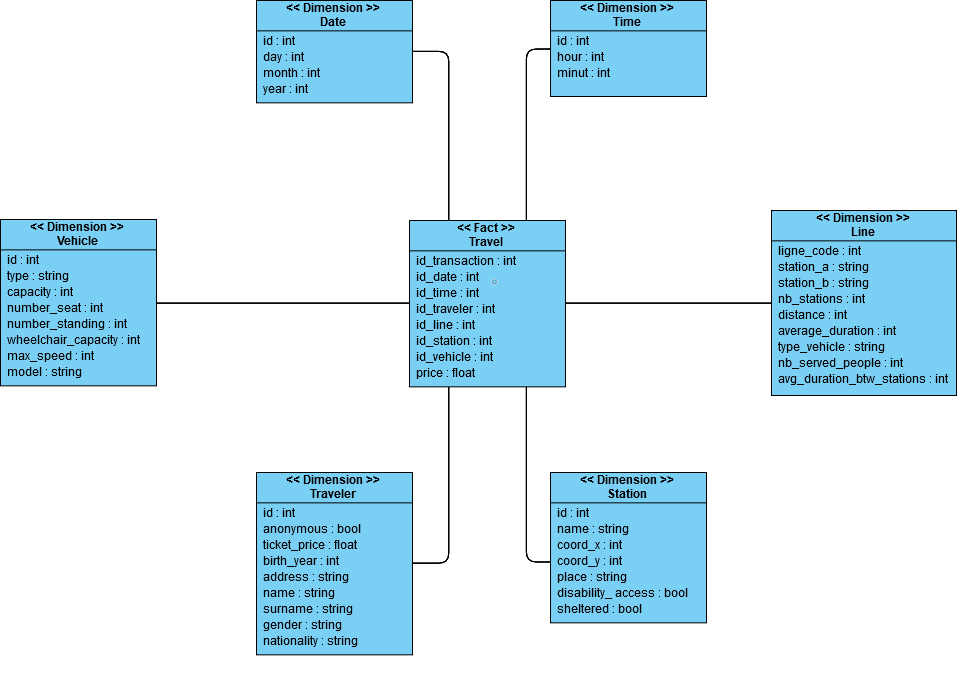
\includegraphics[scale=0.65]{images/voyages_datamart.png}
  \caption{modèle en étoile de l'action \og voyages \fg}
\end{figure}

Les mesures de la table des voyages sont :
\begin{itemize}
  \item \texttt{travel\_price} : additive
\end{itemize}

\newpage

\subsection*{\textit{Data Mart} de \og maintenance \fg}
\label{subsec:data_mart_maintenance}
\addcontentsline{toc}{subsection}{\nameref{subsec:data_mart_maintenance}}
\begin{figure}[!ht]
  \centering
  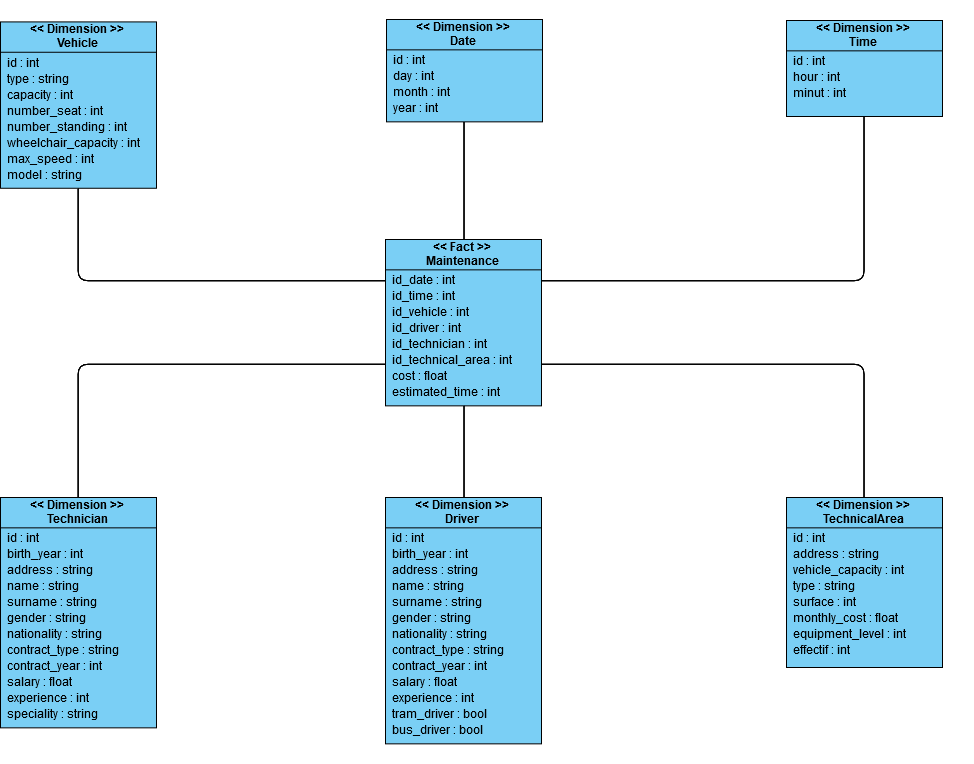
\includegraphics[scale=0.65]{images/maintenance_datamart.png}
  \caption{modèle en étoile de l'action \og maintenance \fg}
\end{figure}

Les mesures de la table des maintenances sont :
\begin{itemize}
  \item \texttt{cost} : additive
  \item \texttt{estimated\_time} : additive
\end{itemize}

\newpage

\subsection*{\textit{Data warehouse} de \textit{tam-voyages}}
\label{subsec:data_warehouse}
\addcontentsline{toc}{subsection}{\nameref{subsec:data_warehouse}}
\begin{figure}[!ht]
  \centering
  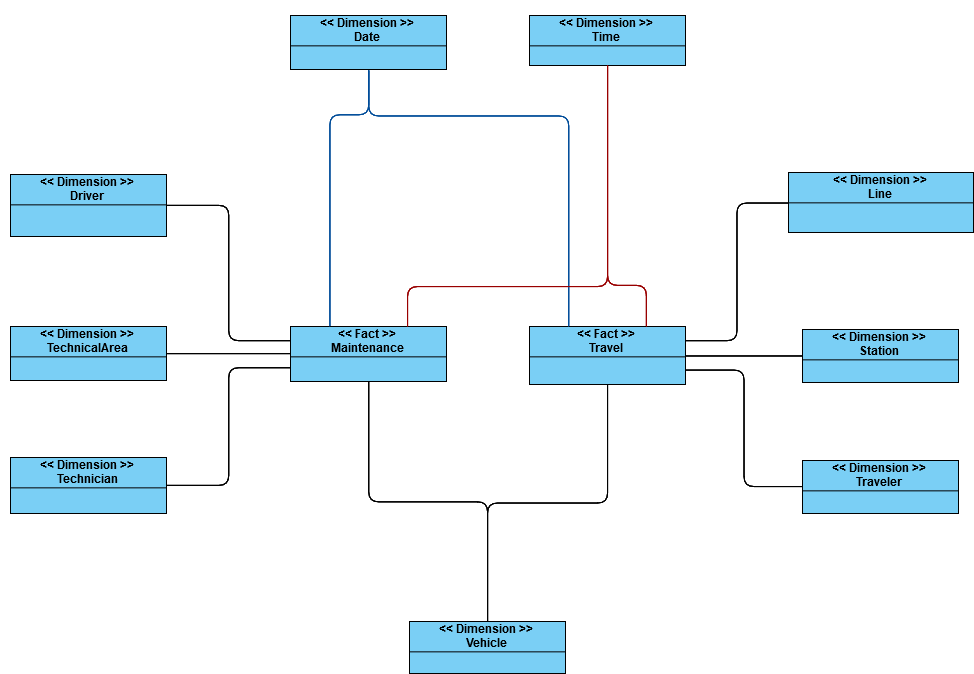
\includegraphics[scale=0.6]{images/data_warehouse.png}
  \caption{le \textit{data warehouse} résultant}
\end{figure}

\newpage

\section*{Question 7}
\label{sec:question_7}
\addcontentsline{toc}{section}{\nameref{sec:question_7}}

\section*{Question 8}
\label{sec:question_8}
\addcontentsline{toc}{section}{\nameref{sec:question_8}}

\end{document}
